\documentclass[10pt,a4paper]{article}
\usepackage[utf8]{inputenc}
\usepackage{amsmath}
\usepackage{amsfonts}
\usepackage{amssymb}
\usepackage{tikz}
\usepackage{graphicx}
\author{James Lee}
\title{10th Assignment of Computational Physics}
\begin{document}
	\maketitle
	\begin{abstract}
		In this report I present to you the numerical solution to Problem 3.26.
	\end{abstract}
	\section{Introduction}
	This program aims to investigate the chaotic behavior of Lorenz model using Euler method.\\
	The Lorenz system is a system of ordinary differential equations (the Lorenz equations, note it is not Lorentz) first studied by Edward Lorenz. It is notable for having chaotic solutions for certain parameter values and initial conditions. In particular, the Lorenz attractor is a set of chaotic solutions of the Lorenz system which, when plotted, resemble a butterfly or figure eight.\\
	In 1963, Edward Lorenz developed a simplified mathematical model for atmospheric convection. The model is a system of three ordinary differential equations now known as the Lorenz equations:
	\begin{align}
		\frac{\mathrm{d}x}{\mathrm{d}t} &= \sigma (y - x), \\
		\frac{\mathrm{d}y}{\mathrm{d}t} &= -xz+rx - y, \\
		\frac{\mathrm{d}z}{\mathrm{d}t} &= x y - bz.
	\end{align} 
	From a technical standpoint, the Lorenz system is nonlinear, three-dimensional and deterministic. When the parameters are given particular values, Lorenz model behaves as a chaotic system.\\
	It is not very easy to solve this ODE analytically. In order to investigate its motion, we trun to numerical solutions.
	
    \section{Main Content}
    \subsection{Chaotic Behavior}
    In order to give a numerical solution, one should fix the parameters numerically at first:
    \begin{align}
    b&=\frac{8}{3}\\
    \sigma&=0.5
    \end{align}
    the initial conditions:
    \begin{align}
    x&=1\\
    y&=z=0
    \end{align} 
    Investigations show that parameter $r$ plays a role that is similar to $F_D$'s role in pendulum's case. Therefore, we will investigate Lorenz model's behavior as $r$ varies.\\   
    The numerical solution to this case will be plotted in figure.1.
    \begin{figure}[htbp]
    	\centering
    	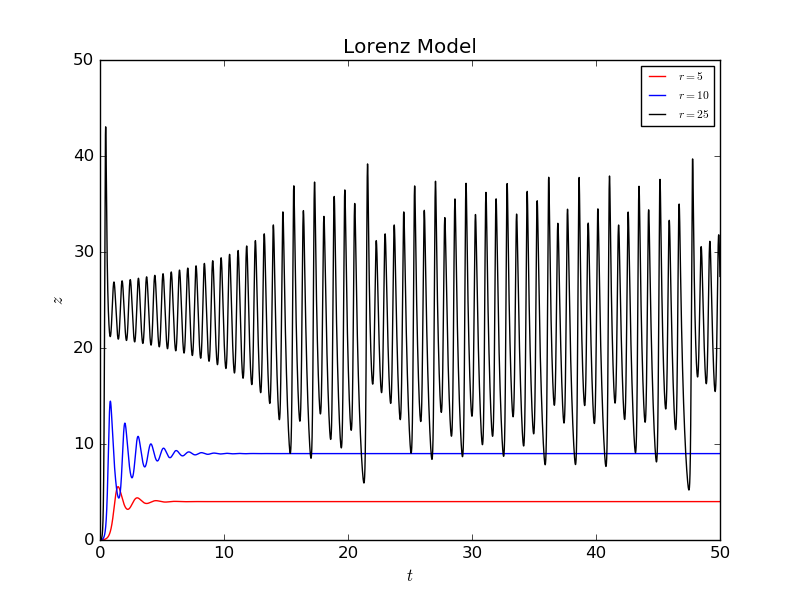
\includegraphics[width=5in]{Lorenz_1.png}
    	\caption{$z-t$ relation with different value of $r$}
    \end{figure}
    As we can see in the numerical plot figure, when $r$ (the driven force) is relatively small, the Lorenz system's behaviors are very much alike to normal linear oscillators. However, when $r$ (the driven force) is relatively large, the Lorenz system's motion becomes peculiar. Such motions are named \emph{chaotic motion}.\\
    We should recall that chaotic behavior begins at a threshold ''Driven Force''. Theoretically, in our case, the threshold is $r=24.74$. Therefore, it is no wonder that $r=25$ case behaves chaotically.\\
    In the following discussions, I will investigate $r=25$ case.
    
   \subsection{Phase Space and Poincare Section}
   Chaotic motion also has its appearance in the phase space.\\
   In the figure.2, I will plot the $z-x$ curve.
   \begin{figure}[htbp]
   	\centering
   	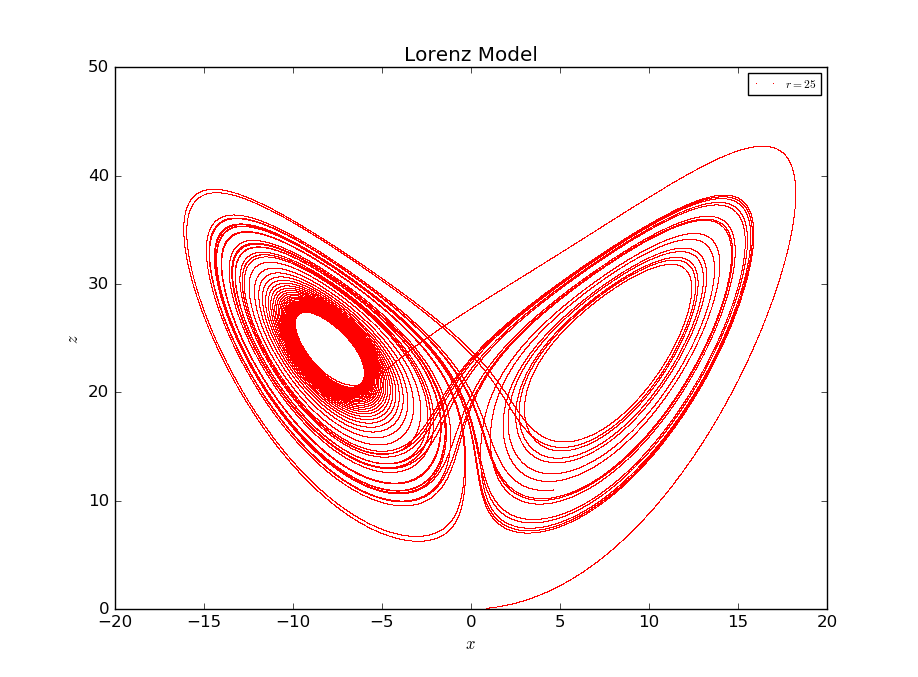
\includegraphics[width=4in]{Lorenz_2.png}
   	\caption{Trajectory on the $x-z$ Plane}
   \end{figure}
   As we can see from this trajectory, the chaotic motion has underlying regularity in irregularity. In order to conduct further investigations, I will plot the Poincare sections in this case.
    \begin{figure}[htbp]
    	\centering
    	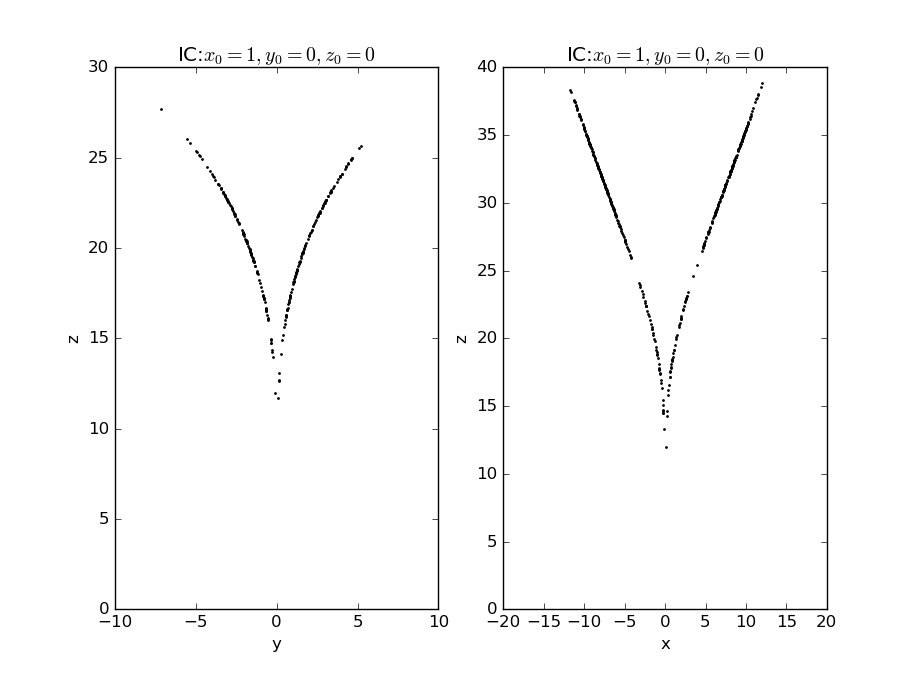
\includegraphics[width=5in]{Lorenz_7.png}
    	\caption{Trajectory on the $x-z$ Plane with the Previous Initial Condition}
    \end{figure}
    The Poincare section is plotted in figure.3. I should further remark that these two Poincare sections are invariant under change of initial condition.\\
    Another plot of Poincare sections with different initial conditions are plotted in figure.4.
    \begin{figure}[htbp]
    	\centering
    	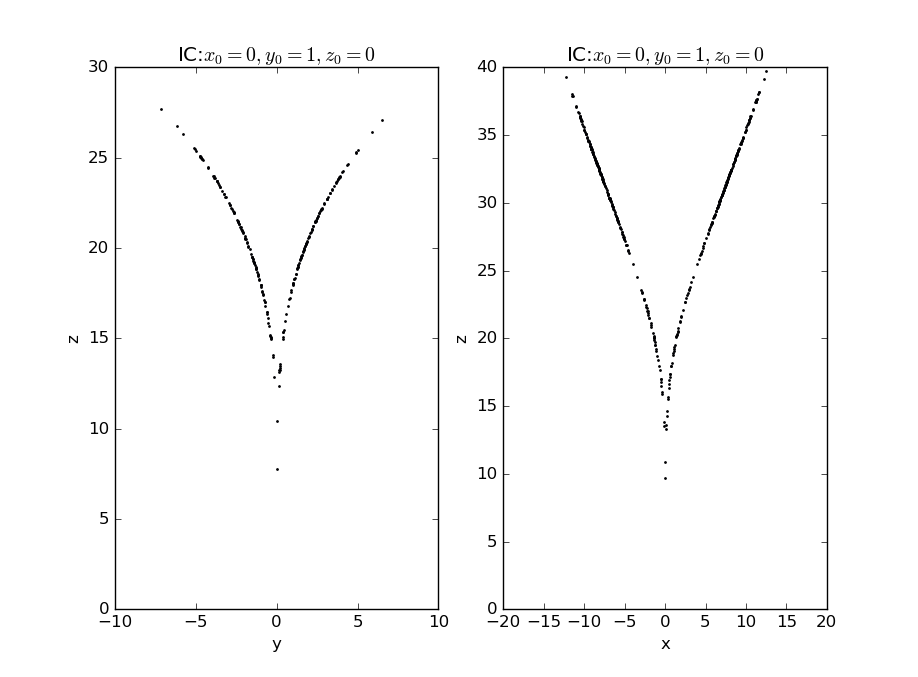
\includegraphics[width=5in]{Lorenz_6.png}
    	\caption{Trajectory on the $x-z$ Plane with New Initial Condition}
    \end{figure}
    As we can see from the figures, the two sets of Poincare sections with different IC are practically the same, which agrees with our theoretical predictions.
    
    \subsection{Routes to Chaos}
    The Lorenz model exhibits the period-doubling routes to chaos. Theoretical predictions yield that when $r=160$, the Lorenz system's motion is periodic(not chaotic). However, as we shall see in numerical calculations, small deviation from $r$ can cause the periodicity to flee. The numerical simulation is plotted in figure.5.\\
    We further remark on the plot that $r=163.8$ curve's amplitude is not two times the $r=160$ case. The reason I lift it up is that I seek a visual distinction between the two curves.\\
    As we can see in the plot, the numerical simulation confirms theoretical predicitions.
    \begin{figure}[htbp]
    	\centering
    	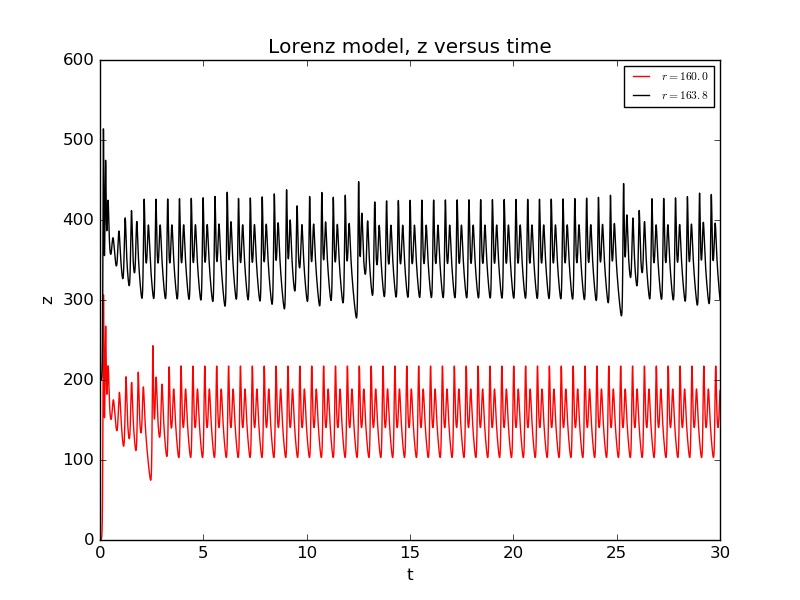
\includegraphics[width=5in]{Lorenz_4.png}
    	\caption{Routes to Chaos}
    \end{figure}
    \section*{Acknowledgement}
    When tackling this assignment, I benefitted a lot from the valuable discussions with Liu Xingchen. I would like to thank him for pointing out several syntax errors I made, also, for his willingness to discuss with me.
    
    \begin{thebibliography}{99}
    	\bibitem{}Hunter J, the Matplotlib Documentation, 2016
    	\bibitem{}Giordano N.J, Nakanishi H, Computational Physics, Pearson Education, 2007
    \end{thebibliography} 
\end{document}